% ISEF Project Presentation -- Mathematics / Computer Science template.
% 12 landscape pages, exported as images. Constraints observed: 14pt body
% (the stated minimum; rendered at image scale it reads well above that);
% no animation; no active hyperlinks (hyperref deliberately not loaded); no
% contact details, logos or QR codes; references confined to one page.
% All counts and thresholds come from zf_numbers.tex, generated by
% verification/verify_all.py from the certificates on disk.
\documentclass[aspectratio=169,14pt]{beamer}
\usetheme{default}
\usepackage[T1]{fontenc}
\usepackage{amsmath,amssymb,booktabs,graphicx}
% GENERATED by verification/verify_all.py -- do not edit by hand.
% Every number here is read off the certificates on disk.

\newcommand{\NtileThree}{23}
\newcommand{\LvalThree}{21}
\newcommand{\LmaxThree}{43}
\newcommand{\NtileFour}{33}
\newcommand{\LvalFour}{29}
\newcommand{\LmaxFour}{61}
\newcommand{\NtileFive}{21}
\newcommand{\LvalFive}{54}
\newcommand{\LmaxFive}{75}
\newcommand{\NtileThreeFour}{56}
\newcommand{\NtileAll}{77}
\newcommand{\SettleThree}{21}
\newcommand{\SettleFour}{29}
\newcommand{\SettleFive}{162}
\newcommand{\NcertGN}{17}
\newcommand{\GNlo}{17}
\newcommand{\GNhi}{33}
\newcommand{\MaxAlpha}{1.0\times10^{-9}}
\newcommand{\RamLastOne}{14}
\newcommand{\RamCountOne}{9}
\newcommand{\RamLastTwo}{23}
\newcommand{\RamCountTwo}{19}
\newcommand{\RamLastThree}{32}
\newcommand{\RamCountThree}{18}
\newcommand{\RamLastFour}{42}
\newcommand{\RamCountFour}{34}
\newcommand{\RamLastFive}{50}
\newcommand{\RamCountFive}{28}
\newcommand{\RamLastSix}{49}
\newcommand{\RamCountSix}{20}
\newcommand{\RamLastSeven}{70}
\newcommand{\RamCountSeven}{39}
\newcommand{\RamLastEight}{49}
\newcommand{\RamCountEight}{16}
\newcommand{\RamLastNine}{90}
\newcommand{\RamCountNine}{50}
\newcommand{\RamLastTen}{52}
\newcommand{\RamCountTen}{14}
\newcommand{\RamTotal}{247}
\newcommand{\RamKmax}{10}
\newcommand{\RamCases}{458}
\newcommand{\RamBoundTwo}{23}
\newcommand{\RamBoundThree}{32}
\newcommand{\RamBoundFour}{42}
\newcommand{\RamDirichlet}{231}
\newcommand{\RamAllTotal}{460}
\newcommand{\RamAllIso}{324}
\newcommand{\RamAllMaxN}{112}
\newcommand{\RamAllMaxK}{45}
\newcommand{\RamAllSizes}{80}
\newcommand{\RamAllCases}{13110}
\newcommand{\RatClassTwo}{7,9,15,20}
\newcommand{\RatClassThree}{10,24,42}
\newcommand{\RatClassFour}{60,70,90}
\newcommand{\RatClassFive}{24,126}
\newcommand{\RatClassSix}{\text{none}}
\newcommand{\RatClassSeven}{120}
\newcommand{\TileAllK}{9}
\newcommand{\Nchecks}{150}


\definecolor{myblue}{RGB}{18,52,102}
\definecolor{mymid}{RGB}{42,86,150}
\definecolor{mylight}{RGB}{226,234,246}

\setbeamercolor{frametitle}{fg=white,bg=myblue}
\setbeamercolor{structure}{fg=myblue}
\setbeamertemplate{navigation symbols}{}
% A frametitle band that wraps long titles without eating the frame body.
% Two earlier attempts failed: a fixed ht= clipped a two-line title to its last
% line, and combining wd=\paperwidth with leftskip/rightskip/sep silently
% pushed the whole body off the slide (the references page rendered blank).
% Padding goes INSIDE the box, and the box keeps beamer's own width.
\setbeamertemplate{frametitle}{%
  \nointerlineskip
  \begin{beamercolorbox}[wd=\paperwidth]{frametitle}%
    \vspace{0.30em}%
    \hspace{0.7em}\begin{minipage}{0.93\paperwidth}\raggedright
      \strut\insertframetitle\strut
    \end{minipage}%
    \vspace{0.30em}%
  \end{beamercolorbox}}
\setbeamerfont{frametitle}{series=\bfseries}
\setbeamertemplate{footline}{%
  \hfill\color{gray}\tiny\insertframenumber/12\hspace{0.8em}\vspace{0.25em}}
\setbeamertemplate{blocks}[rounded]
\setbeamercolor{block title}{fg=white,bg=mymid}
\setbeamercolor{block body}{bg=mylight}
% reclaim the default padding around blocks -- three slides ran half a line long
\addtobeamertemplate{block begin}{\vspace{-0.5em}}{}
\addtobeamertemplate{block end}{}{\vspace{-0.6em}}
\setbeamersize{text margin left=1.1em,text margin right=1.1em}
\graphicspath{{figures/}}

\newcommand{\key}[1]{\textcolor{myblue}{\textbf{#1}}}
\newcommand{\kb}[1]{\begin{center}\colorbox{mylight}{\parbox{0.94\textwidth}{#1}}\end{center}}

\begin{document}

%% ------------------------------------------------------------- 1. TITLE
\begin{frame}[plain]
\vfill
\begin{center}
{\color{myblue}\bfseries\large
Where Optimal Networks Stop Existing\\[0.25em]
Certified Spectral Limits of Cyclic Architectures\par}
\vspace{1.0em}
Category: Mathematics \qquad Project ID: \rule{3cm}{0.4pt}
\end{center}
\vfill
\kb{\centering Every graph has a zeta function, so every graph has a Riemann
Hypothesis --- and unlike the classical one, it can be \key{decided}. We decide
it \key{completely and in exact arithmetic} for the generalized Petersen graphs,
and prove that only \key{finitely many} satisfy it.}
\vfill
\end{frame}

%% ------------------------------------------------------- 2. INTRODUCTION
\begin{frame}{INTRODUCTION --- an RH you can decide}
\key{Every graph has a zeta function.} The \key{Ihara zeta}
$\zeta_X(u)=\prod_{[C]}(1-u^{\ell(C)})^{-1}$, over primitive closed geodesics,
has an Euler product, a functional equation, and a \key{prime number theorem}.

\key{So one can ask the RH for a graph:} do the poles of $\zeta_X(q^{-s})$ in
the critical strip lie on $\mathrm{Re}\,s=\tfrac12$?

\key{And here it is decidable.} By the Ihara determinant formula, a
$(q+1)$-regular graph satisfies the RH \emph{iff} it is \key{Ramanujan}: every
eigenvalue with $|\lambda|\ne q+1$ has $|\lambda|\le2\sqrt q$.

\kb{$2\sqrt q$ is the smallest gap any infinite family can have: the
\key{optimal expanders}.}
\end{frame}

%% -------------------------------------------------- 3. INTRODUCTION cont.
\begin{frame}{INTRODUCTION --- the question}
\kb{\centering\key{For which $n$ and $k$ does $P(n,k)$ satisfy the Riemann
Hypothesis?}}

\key{A question of a recognised kind.} The same classification exists for
unitary Cayley graphs (Droll) and integral circulants (Le--Sander) --- only
\emph{finitely many} members qualify.

\key{The ingredients have been on the shelf since 2011.} Gera and St\u{a}nic\u{a}
determined the spectrum of $P(n,k)$ completely --- but their paper contains
\key{no occurrence} of \emph{Ramanujan}, \emph{expander} or \emph{spectral gap}.

\key{And it is not just a computation.} At a band edge the decision compares
nested radicals, where floating point does not decide --- it guesses.
\end{frame}

%% --------------------------------------------------------- 4. FRAMEWORK
\begin{frame}{FRAMEWORK --- a symbol on a grid}
$P(n,k)$ is a \key{cyclic cover}: it carries the rotation $\rho:i\mapsto i+1$,
so the adjacency matrix decomposes over the characters of $\mathbb Z_n$:
\[
  M_j=\begin{pmatrix}\alpha_j&1\\1&\beta_j\end{pmatrix},\qquad
  \alpha_j=2\cos\tfrac{2\pi j}{n},\quad\beta_j=2T_k(\alpha_j/2).
\]
\key{On the zeta side this is the factorization} into Artin--Ihara
$L$-functions.

\kb{So the spectrum is \key{one fixed curve sampled at $n$ points}, and the RH
holds when no sample lands where the curve is too big. \key{Does the grid miss
the bad bands?} It refines as $n$ grows --- which will bound $n$.}
\end{frame}

%% ----------------------------------------- 5. FINDINGS 1 -- the criterion
\begin{frame}{FINDINGS 1 --- clearing the radicals}
Eigenvalues $\bigl(A\pm\sqrt{(\alpha-\beta)^2+4}\bigr)/2$ against $2\sqrt2$:
\key{two nested irrationalities}. Substituting $\lambda=\pm2\sqrt2$ into $\lambda^2-A\lambda+(P-1)$ gives
$2\sqrt2|A|\le7+P$. Squaring twice removes both radicals, and \key{each squaring
is an equivalence}: $|A|\le4<4\sqrt2$, $|P|\le4$.

\kb{\key{Criterion.} $P(n,k)$ satisfies the RH iff
\[D_k(u)=\bigl(7+4uT_k(u)\bigr)^2-8\bigl(2u+2T_k(u)\bigr)^2\ \ge\ 0\]
at $u=\cos\frac{2\pi j}{n}$ for every non-trivial $j$.}

The poles of a zeta function: now \key{one integer polynomial}.
\end{frame}

%% ---------------------------------------- 6. FINDINGS 2 -- finiteness
\begin{frame}{FINDINGS 2 --- finiteness}
Everything follows from three \key{exact} evaluations:
\[
  D_k(1)=-7,\quad D_k(0)\ge17,\quad
  D_k(-1)=-7\ (k\text{ odd}),\ +9\ (k\text{ even}).
\]
$D_k(1)<0$ puts a \key{forbidden band at $u=1$}, where the grid accumulates.
With $s=(1-\cos t)+(1-\cos kt)$, AM--GM gives $4ab\le s^2$, and
$s^2+(4\sqrt2-4)s$ hits $8\sqrt2-11$ \key{exactly} at $s=(\sqrt2-1)^2$; then
$1-\cos\theta\le\theta^2/2$ bounds $t$.

\kb{\key{Theorem --- for every $k$.} $n\le\pi(2+\sqrt2)\sqrt{k^2+1}$. No
expansion, no computation. Per $k$ the exact root sharpens this to
$B_k=2\pi/\arccos u_k$, \key{sharp at $k=2,3,4$}.}
\end{frame}

%% ---------------------------------------- 7. FINDINGS 3 -- the parity law
\begin{frame}{FINDINGS 3 --- a parity law}
For \emph{odd} $k$, $D_k(-1)=-7<0$: a \key{second band at $t=\pi$}. For even
$k$, $D_k(-1)=+9>0$ and there is none.

\key{But the grid meets $t=\pi$ only when $n$ is even} --- and there the sample
is the $-3$ of a \emph{bipartite} graph, which the Ramanujan condition
\key{exempts}. Odd $n$ lands just short, inside the band.

\kb{\key{Theorem (parity law).} At $t=\pi$ the same algebra returns the
\emph{identical} expression, so odd $n$ is cut at \key{exactly half} the same
constant. \key{Sharp at $k=1,5,7,9$.}}

\key{Being bipartite helps} --- worth a factor of two in $n$.
\end{frame}

%% ------------------------------------ 8. FINDINGS 4 -- exact certification
\begin{frame}{FINDINGS 4 --- a theorem for $k\le9$, exact arithmetic beyond}
\key{Theorem (closed form).} For $k\in\{1,2,3,4,5,7,9\}$ the negative set of
$D_k$ on $[-1,1]$ is the end band(s) alone --- Sturm's theorem on one integer
polynomial --- so only the grid point $j=1$ (and, for odd $n$ and odd $k$,
$j=\tfrac{n-1}{2}$) can fail:
\[
  P(n,k)\ \text{Ramanujan}\iff 2k<n\le B_k,\quad\text{and }n\le B_k/2\text{ if }n,k\text{ odd}.
\]
From $k=10$ on an interior band always appears, and the list has gaps.

\kb{\key{Beyond $k=9$:} $D$ is an algebraic integer of $\mathbb Z[\zeta_m]$,
decided exactly mod $\Phi_m$ --- a finite check after a theorem made the problem finite.}
\end{frame}

%% -------------------------------------- 9. FINDINGS 5 -- the classification
\begin{frame}{FINDINGS 5 --- the complete classification}
\begin{center}
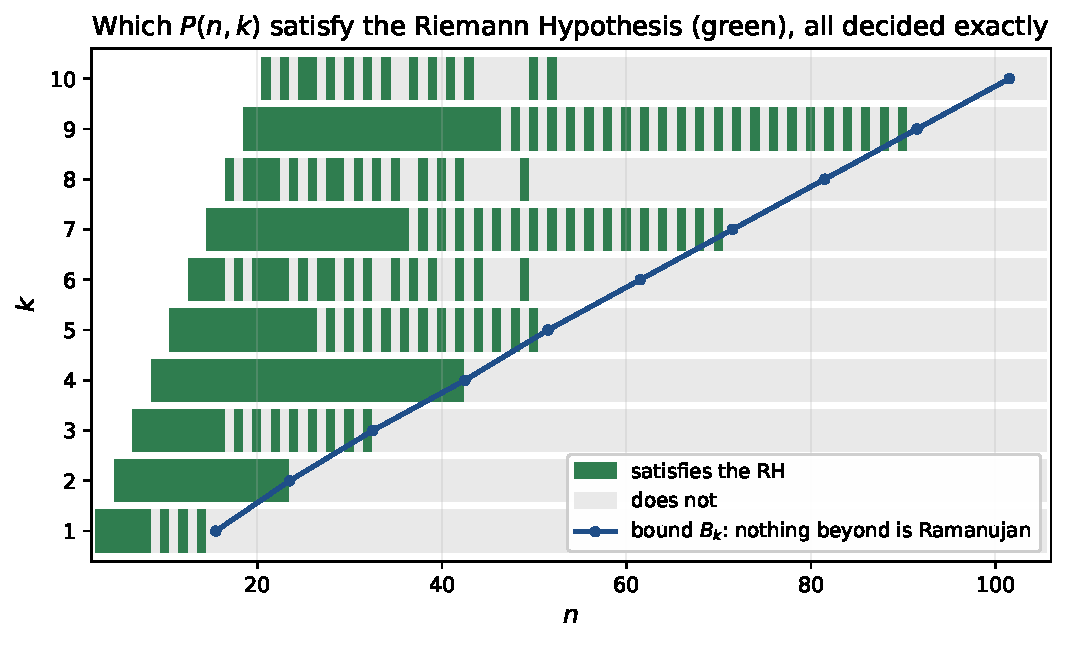
\includegraphics[width=0.52\textwidth]{fig_ramclass.pdf}
\end{center}
\vspace{-0.9em}
\kb{\key{Theorem.} Every $n$, \emph{every} $k$: exactly \key{$\RamAllTotal$}
pairs satisfy the RH ($\RamAllIso$ up to isomorphism), from $\RamAllCases$ cases
in \key{exact arithmetic}. Nothing past $k=\RamAllMaxK$ qualifies.}
\end{frame}

%% ------------------------------------ 10. FINDINGS 6 -- the same engine
\begin{frame}{FINDINGS 6 --- the same engine}
The same decomposition settles the \key{inverse eigenvalue problem} here: over
\emph{every} matrix carrying the pattern, eliminating the inner coordinates
leaves one recurrence of order $2k+2$, so $\operatorname{null}A\le2k+2$.

\key{That ceiling equals the best known upper bound on $Z$} --- so the method
either settles it completely or cannot settle it at all.

\kb{Building the matrix from interchangeable \key{tiles} turns an all-$n$ claim
into finitely many finite ones. Certifying $\NtileAll$ tiles exactly gives
$Z(P(n,k))=M(P(n,k))=2k+2$ for \key{every} $n$ at $k=2,3,4$ --- proving
\key{Conjecture 5} of a 2026 note.}
\end{frame}

%% --------------------------------------------------------- 11. CONCLUSIONS
\begin{frame}{CONCLUSIONS}
\key{How this answers the question.} Clearing the radicals gives one integer
polynomial; it factors into a form with \emph{no $k$ in it}; Dirichlet bounds
$n$ uniformly in $k$; for $k\le9$ ($k\ne6,8$) the answer is a theorem, and the
finite remainder is decided in exact arithmetic.

\key{Proved:} criterion, corner form, finiteness, parity, closed form,
ceiling, symbol classification, tiling, the leading-coefficient criterion. \key{Finite exact checks:} the census
for $k\ge10$, small $Z$. \key{One computer-assisted existence proof:} the tiles.

\key{Open.} $M(P(24,4))$; an effective $L(k)$ and a tile at $k\ge6$; the
cover ceiling when $c_{\max}$ has two monomials; a hand proof of tile existence.
\end{frame}

%% ---------------------------------------------------------- 12. REFERENCES
\begin{frame}{REFERENCES \& ACKNOWLEDGEMENTS}
\begin{enumerate}\setlength\itemsep{0pt}
\item Terras, \emph{Zeta Functions of Graphs}, CUP (2010); \emph{Zeta
      Functions and Chaos}, notes (2009), Ex.\ 9.
\item Lubotzky, Phillips, Sarnak, \emph{Combinatorica} 8 (1988) 261--277.
\item Gera, St\u{a}nic\u{a}, \emph{Australas.\ J. Combin.} 49 (2011) 39--45.
\item Le, Sander, \emph{Electron.\ J. Combin.} 20 (2013) \#P35.
\item Krishnan, arXiv:2607.19412 (2026).
\item Rashidi et al., \emph{JACODESMATH} 7 (2020) 183--193.
\item AIM Minimum Rank Work Group, \emph{LAA} 428 (2008) 1628--1648.
\item Niven, \emph{Irrational Numbers}, Carus Monographs 11 (1956).
\end{enumerate}
\key{Acknowledgements.} All mathematics, code and computation are my own.
\end{frame}

\end{document}
